\documentclass[a4paper]{article}

\usepackage[english]{babel}
\usepackage[utf8]{inputenc}
\usepackage{amsmath}
\usepackage{graphicx}
\usepackage{color}
\usepackage{float}
\usepackage{listings}
\definecolor{keywords}{RGB}{255,0,90}
\definecolor{comments}{RGB}{0,0,113}
\definecolor{red}{RGB}{160,0,0}
\definecolor{green}{RGB}{0,150,0}
\definecolor{codegreen}{rgb}{0,0.6,0}
\definecolor{codegray}{rgb}{0.5,0.5,0.5}
\definecolor{codepurple}{rgb}{0.58,0,0.82}
\definecolor{backcolour}{rgb}{0.95,0.95,0.92}
\definecolor{brown}{rgb}{0.59, 0.29, 0.0}
\definecolor{beaublue}{rgb}{0.74, 0.83, 0.9}
\definecolor{orange}{rgb}{1.0, 0.5, 0.0}
\definecolor{darkslategray}{rgb}{0.18, 0.31, 0.31}
\definecolor{deepblue}{rgb}{0,0,0.5}
\definecolor{deepred}{rgb}{0.6,0,0}
\definecolor{deepgreen}{rgb}{0,0.5,0}
\definecolor{auburn}{rgb}{0.43, 0.21, 0.1}
\definecolor{bistre}{rgb}{0.24, 0.17, 0.12}
\definecolor{babyblue}{rgb}{0.54, 0.81, 0.94}
\definecolor{ballblue}{rgb}{0.13, 0.67, 0.8}
\lstdefinestyle{myMatlabstyle}{
	language=Matlab,
	backgroundcolor=\color{white},   
	commentstyle=\color{deepgreen},
	keywordstyle=\color{black},
	identifierstyle=\color{black},
	numberstyle=\tiny\color{codegray},
	stringstyle=\color{purple},
	basicstyle=\footnotesize,
	breakatwhitespace=false,         
	breaklines=true,                 
	captionpos=b,                    
	keepspaces=true,                 
	numbers=left,                    
	numbersep=5pt,                  
	showspaces=false,                
	showstringspaces=false,
	showtabs=false,                  
	tabsize=2
}
\lstdefinestyle{myPythonstyle}{
	language=Python, 
	basicstyle=\ttfamily\small, 
	keywordstyle=\color{blue},
	commentstyle=\color{green},
	stringstyle=\color{red},
	showstringspaces=false,
	identifierstyle=\color{black},
}
\lstset{language=Matlab,frame=single}
\lstset{language=Python,frame=single}
\usepackage[colorinlistoftodos]{todonotes}
\usepackage[scale=0.75]{geometry}
	\title{Background Separation from Video Streams}

\author{Jithin D. George}

\date{\today}

\begin{document}
\maketitle

\begin{abstract}
Unlike the singular value decomposition, the dynamic mode decomposition makes use of the properties of the fourier transform to incorporate time dynamics into our analysis. As a result, we gain new perspectives and a host of applications like prediction of the future state and here, the ability to obtain the background and foreground from a video.
\end{abstract}

\section{Introduction and Overview}
\label{sec:introduction}


 The Dynamic Mode Decomposition allows us to explore different perspectives into data. Here, we go ahead into separating the background and foreground out of a video after seeing the promising results of \cite{key-2}.
\section{Theoretical Background}
\label{sec:theory}

Given a time series of data, DMD computes a set of modes each of which is associated with a fixed oscillation frequency and decay/growth rate. For linear systems in particular, these modes and frequencies are analogous to the normal modes of the system, but more generally, they are approximations of the modes and eigenvalues of the composition operator (also called the Koopman operator). DMD has recently been extended to include the effect of control to extract low-order models from externally forced or controlled high-dimensional complex systems.The new method of dynamic mode decomposition with control (DMDc) provides the ability to disambiguate between the underlying dynamics and the effects of actuation, resulting in accurate input-output models like explained in \cite{key-1}
\section{Implementation and Development}


Here, we consider two videos. One of the videos is a man walking across the room and the other is a computer generated animation. We use the DMD on them and find the mode with the  $\omega$ closest. This should correspond to the mode that doesn't change with time and thus the background. We then separate the background out to reveal the foreground.


\section{Computational Results}

\subsection{Movement across a room}

The DMD works very well for this case. The original image is shown in \ref{F:Im11}. The background is obtained to a near perfect state as shown with the foreground in \ref{F:Im111}. Since we can't scale the foreground accurately, we can only see the white outline of the person moving across. There seems to be a sort of obstruction towards the end of the videoframes which makes the visibility low. 

\begin{figure}[h] 
	\begin{centering} 
			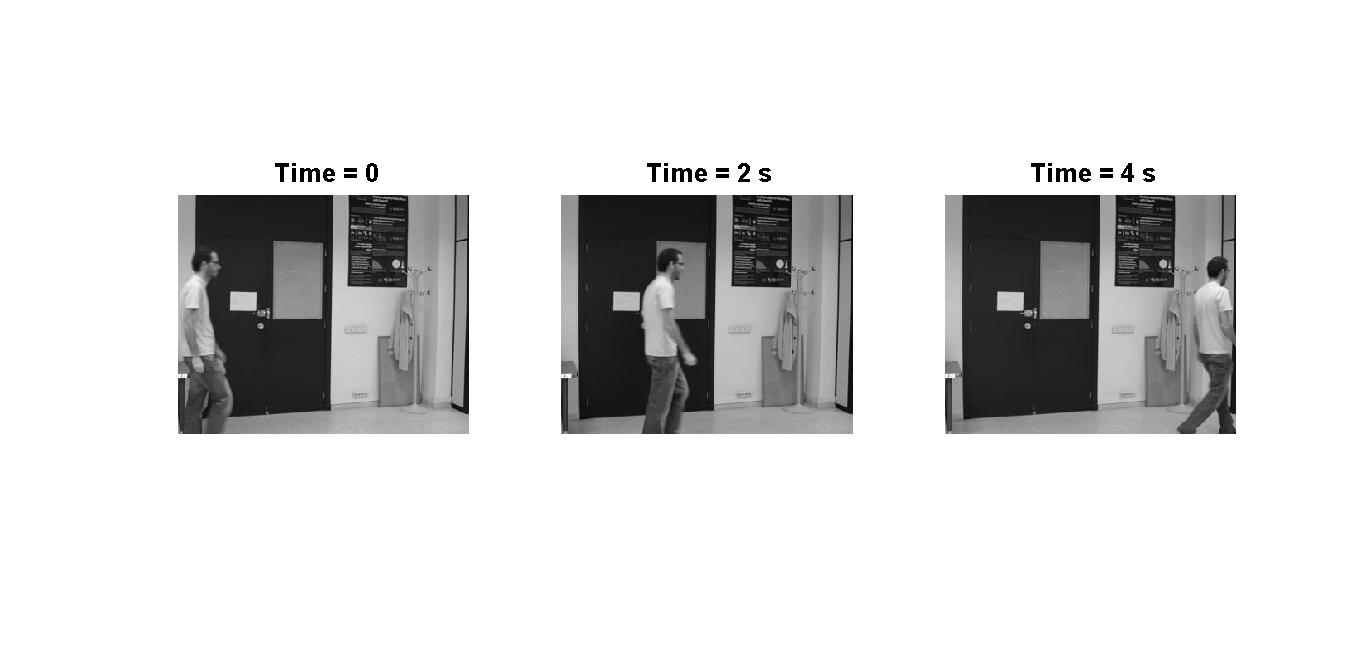
\includegraphics[width=1.1\textwidth]{Im11}
 	\end{centering}
			\caption{Original Image \label{F:Im11}}	
\end{figure}

\begin{figure}[h!] 
	\begin{centering} 
		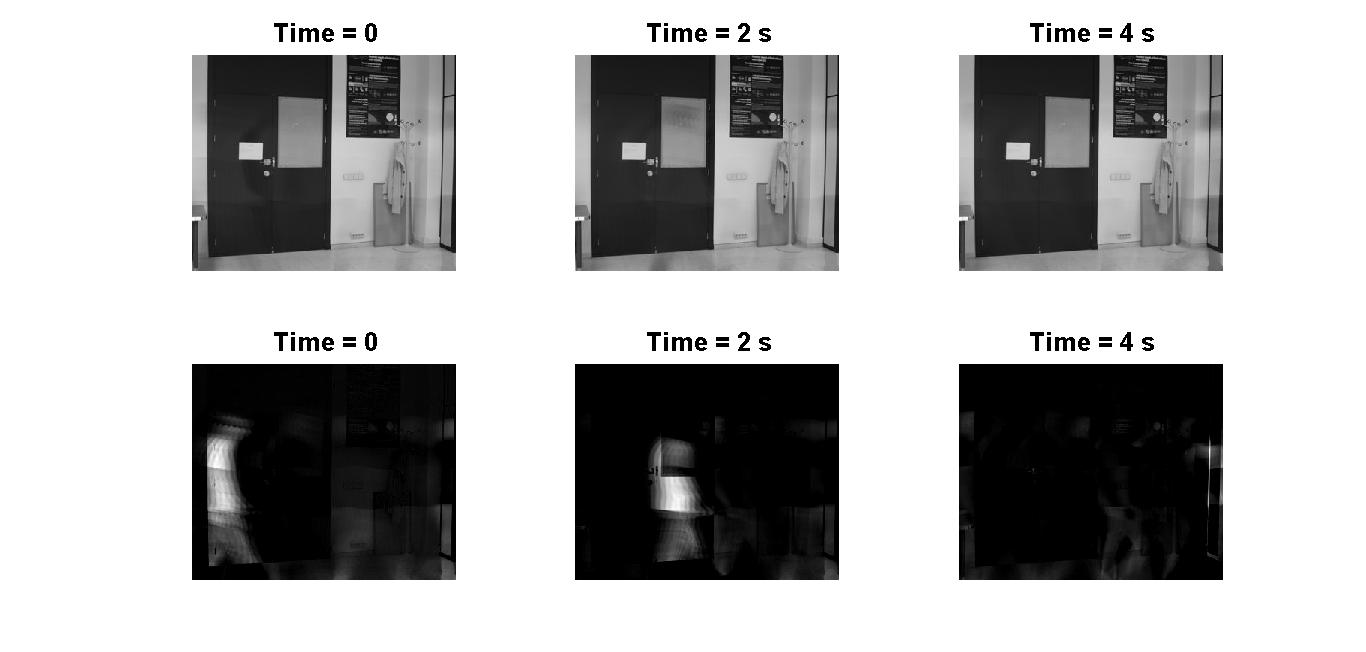
\includegraphics[width=1.1\textwidth]{Image11}
	\end{centering}
	\caption{Background and Foreground \label{F:Im111}}	
\end{figure}

\subsection{Computer generated video}

For this case, the DMD works well for the background. The original image is shown in \ref{F:Im222}. The background is obtained to a near perfect state as shown with the foreground in \ref{F:Im22}. The background is devoid of the moving black car. The foreground however contains trees because they move slightly. The car is missing except for a small light at its position. This is because the car is black in color


\begin{figure}[h] 
	\begin{centering} 
		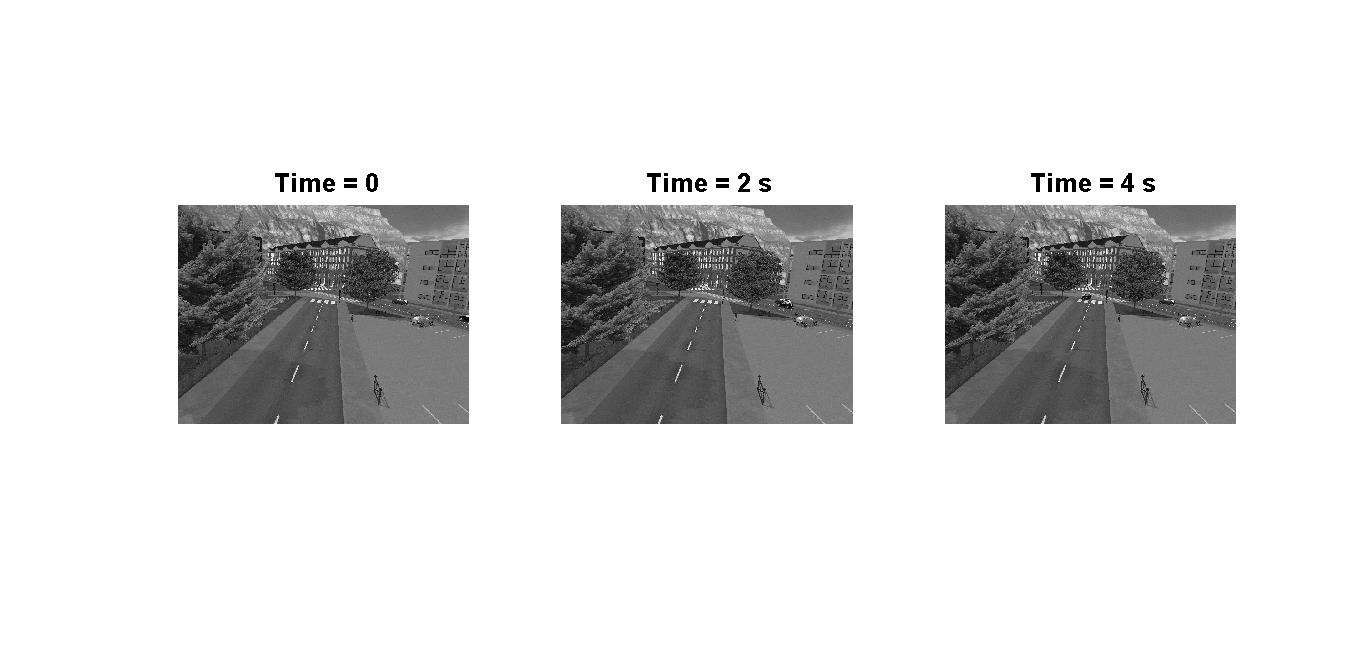
\includegraphics[width=1.1\textwidth]{Im222}
	\end{centering}
	\caption{Original Image \label{F:Im222}}	
\end{figure}

\begin{figure}[h!] 
	\begin{centering} 
		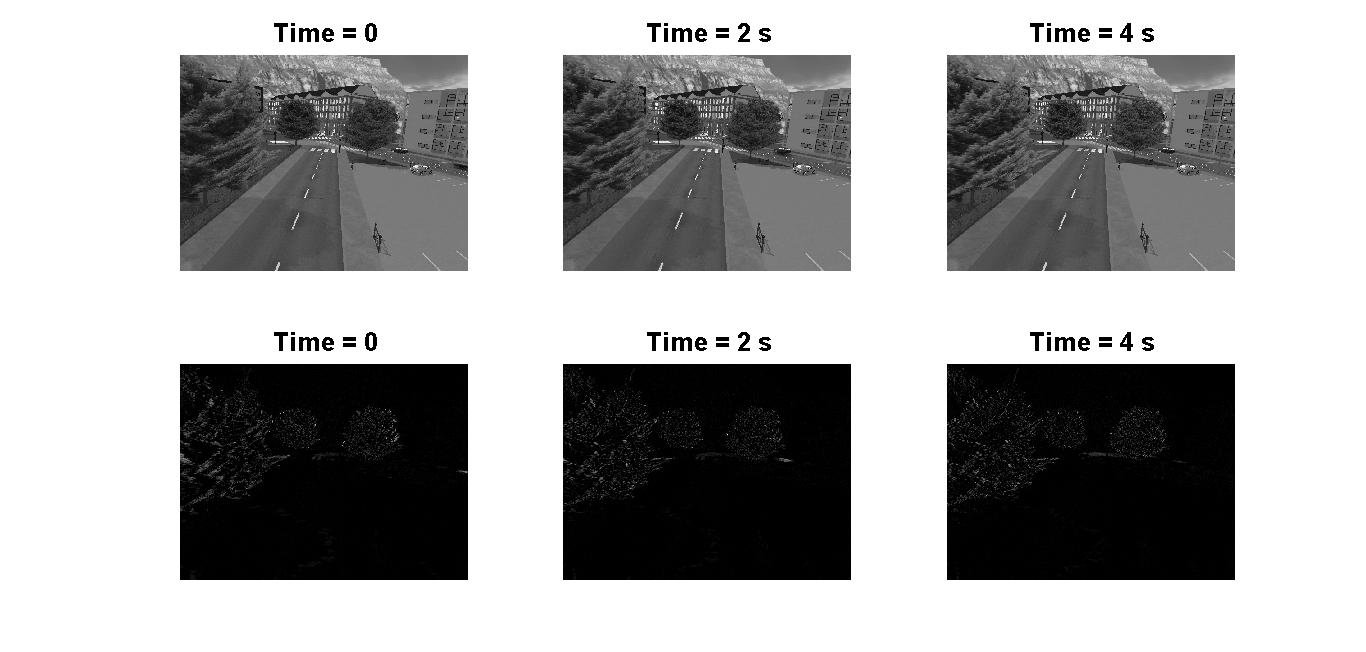
\includegraphics[width=1.1\textwidth]{Image22}
	\end{centering}
	\caption{Background and Foreground \label{F:Im22}}	
\end{figure}

\subsection{Future State Prediction}

We extend the time beyond the length of the videos and show our results in\ref{F:fut}. The result for the moving man is perfect since he is leaving the video. In the animation, the car takes a turn and changes direction. However, there is hardly a few frames in the new direction. So, the future state seems empty because the car seems to vanish behind the tree. Using a few more frames in the new direction and many more modes, we obtain the correct future state in \ref{F:futr}

\begin{figure}[h!] 
	\begin{centering} 
		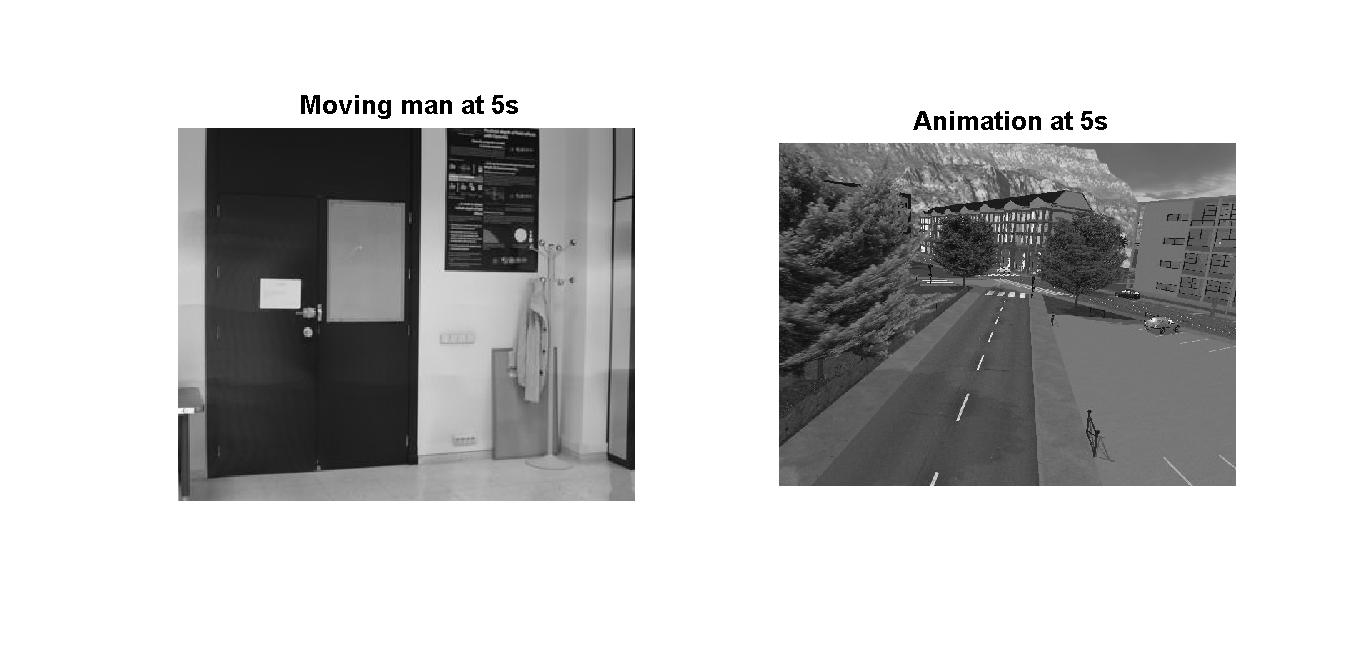
\includegraphics[width=1.1\textwidth]{future}
	\end{centering}
	\caption{Background and Foreground \label{F:fut}}	
\end{figure}

\begin{figure}[h!] 
	\begin{centering} 
		\begin{center}
			
		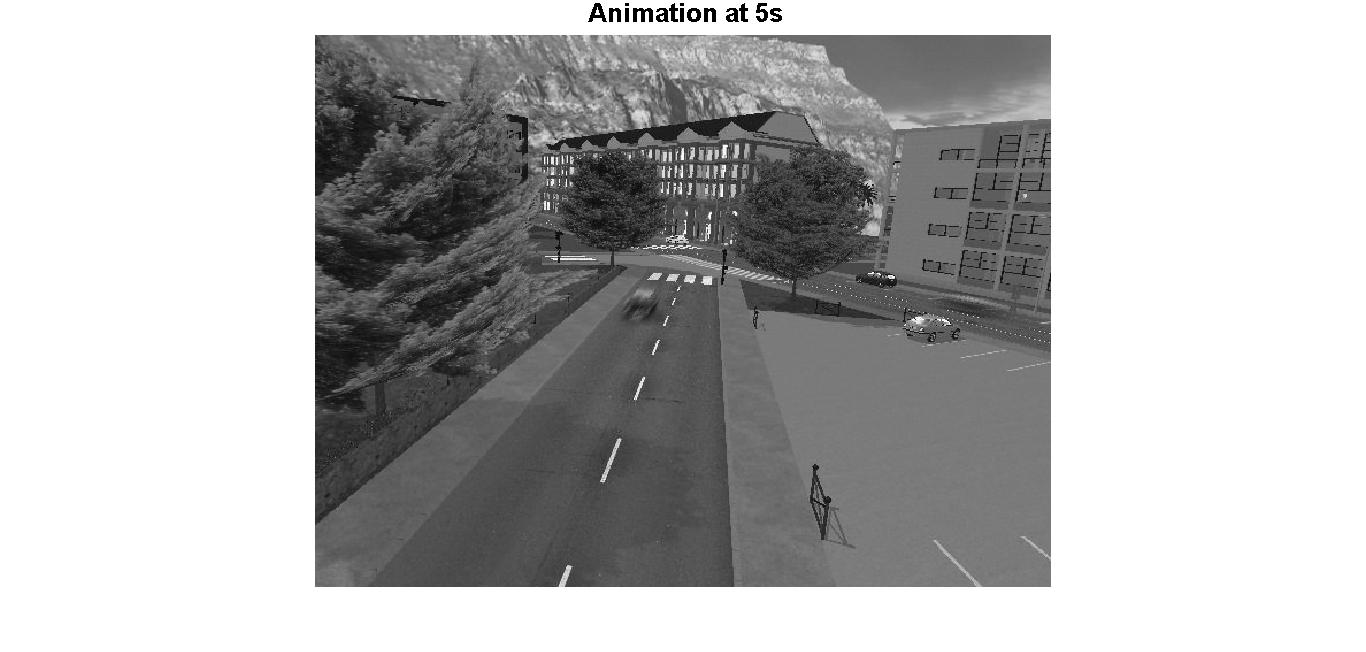
\includegraphics[width=1\textwidth]{futr}
		\end{center}		
	\end{centering}
	\caption{Refined future state \label{F:futr}}	
\end{figure}
\section{Summary and Conclusions}

We obtain the following conclusions
\begin{itemize}
\item The background can be obtained with relative ease in both cases.
\item The DMD shows an incredible ability to predict the future state of the video.
\item Black moving objects are harder to detect.
\item Slightly moving objects like the trees can be detected and affect the imaging.
\item Direction change of the foreground and lack of data in the new direction leads to erroneous future state prediction.
\item Using more modes leads to better clarity and better prediction. 
\end{itemize}

\begin{thebibliography}{1}
	\bibitem{key-1}J. Proctor, S. Brunton and J. N. Kutz, Dynamic mode decomposition with control, arXiv:1409.6358.
	
	\bibitem{key-2}J. Grosek and J. N. Kutz, Dynamic mode decomposition for real-time background/foreground separation in video, arXiv:1404.7592.
	
	

\end{thebibliography}

\newpage

\appendix
%dummy comment inserted by tex2lyx to ensure that this paragraph is not empty


\section{MATLAB Functions used}
\begin{itemize}
\item \textbf{[U,S,V]=svd(A): } \\ This function performs the singular value decomposition of A and returns U,S and V.
\item \textbf{mat2gray(A): } \\ This function converts a matrix to greyscale.

\end{itemize}

\section{MATLAB Code}

\subsection{hw4.m}
\begin{lstlisting}[style=myMatlabstyle]
t=dir;
numFrames = 63;
dt = 3/numFrames;
Y=zeros(288*352,63);
for j=3:numFrames+2
	p= t(j);
	s=p.name;
	X=imread(s);
	X= rgb2gray(X);
	imshow(X); drawnow
	Y(:,j-2)= reshape(X,[288*352,1]);
end

Y2= Y(:,2:end);
Y1= Y(:,1:numFrames-1);
[Phi,omega,lambda,b,Xdmd] = DMD(Y1,Y2,15,dt);



%% DMD reconstruction
mm1 = size(Y1, 2)+10; % mm1 = m - 1
time_dynamics11 = zeros(1, mm1);
b11=b(11,1);
t = (0:mm1-1)*dt; % time vector
for iter = 1:mm1,
	time_dynamics11(:,iter)=(b11.*exp(omega(11,1)*t(iter)));
end;
Phi11= Phi(:,11);
Xdmd11 = Phi11 * time_dynamics11;
ab= Xdmd11(:,20);
abr = reshape(ab,288,352);

abr = mat2gray(real(abr));

Xsparse = Xdmd-abs(Xdmd11);
R= zeros(size(Xsparse));
R(Xsparse<0)= Xsparse(Xsparse<0);
Xback = R+ abs(Xdmd11);
Xsparse = Xsparse- R;
for j = 1:70
	ab= Xsparse(:,j);
	abr = reshape(ab,288,352);
	abr = mat2gray(abs(abr));
	imshow(abr);drawnow
end
\end{lstlisting}
\subsection{plothw4.m}
\begin{lstlisting}[style=myMatlabstyle]
figure;
subplot(1,3,1);
f=20;
A1= reshape(Y(:,1),[dim1,dim2]);
A1g=mat2gray(abs(A1)); 
imshow(A1g);
title('\bf Time = 0','FontSize', f)
subplot(1,3,2);
A2= reshape(Y(:,40),[dim1,dim2]);
A2g=mat2gray(abs(A2)); 
imshow(A2g);
title('\bf Time = 2 s','FontSize', f)
subplot(1,3,3);
A3= reshape(Y(:,90),[dim1,dim2]);
A3g=mat2gray(abs(A3)); 
imshow(A3g);
title('\bf Time = 4 s','FontSize', f)

figure;
subplot(2,3,1);
f=20;
A1= reshape(Xback(:,1),[dim1,dim2]);
A1g=mat2gray(abs(A1)); 
imshow(A1g);
title('\bf Time = 0','FontSize', f)
subplot(2,3,2);
A2= reshape(Xback(:,40),[dim1,dim2]);
A2g=mat2gray(abs(A2)); 
imshow(A2g);
title('\bf Time = 2 s','FontSize', f)
subplot(2,3,3);
A3= reshape(Xback(:,90),[dim1,dim2]);
A3g=mat2gray(abs(A3)); 
imshow(A3g);
title('\bf Time = 4 s','FontSize', f)
% 
subplot(2,3,4);
f=20;
A1= reshape(Xsparse(:,1),[dim1,dim2]);
A1g=mat2gray(abs(A1)); 
imshow(A1g);
title('\bf Time = 0','FontSize', f)
subplot(2,3,5);
A2= reshape(Xsparse(:,40),[dim1,dim2]);
A2g=mat2gray(abs(A2)); 
imshow(A2g);
title('\bf Time = 2 s','FontSize', f)
subplot(2,3,6);
A3= reshape(Xsparse(:,90),[dim1,dim2]);
A3g=mat2gray(abs(A3)); 
imshow(A3g);
title('\bf Time = 4 s','FontSize', f)
\end{lstlisting}
\subsection{DMD.m}
\begin{lstlisting}[style=myMatlabstyle]
function [Phi,omega,lambda,b,Xdmd] = DMD(X1,X2,r,dt)
% function [Phi,omega,lambda,b,Xdmd] = DMD(X1,X2,r,dt)
% Computes the Dynamic Mode Decomposition of X1, X2
%
% INPUTS:
% X1 = X, data matrix
% X2 = X', shifted data matrix
% Columns of X1 and X2 are state snapshots
% r = target rank of SVD
% dt = time step advancing X1 to X2 (X to X')
%
% OUTPUTS:
% Phi, the DMD modes
% omega, the continuous-time DMD eigenvalues
% lambda, the discrete-time DMD eigenvalues
% b, a vector of magnitudes of modes Phi
% Xdmd, the data matrix reconstrcted by Phi, omega, b

%% DMD
[U, S, V] = svd(X1, 'econ');
r = min(r, size(U,2));
U_r = U(:, 1:r); % truncate to rank-r
S_r = S(1:r, 1:r);
V_r = V(:, 1:r);
Atilde = U_r' * X2 * V_r / S_r; % low-rank dynamics
[W_r, D] = eig(Atilde);
Phi = X2 * V_r / S_r * W_r; % DMD modes
lambda = diag(D); % discrete-time eigenvalues
omega = log(lambda)/dt; % continuous-time eigenvalues
%% Compute DMD mode amplitudes b
x1 = X1(:, 1);
b = Phi\x1;

%% DMD reconstruction
mm1 = size(X1, 2)+10; % mm1 = m - 1
time_dynamics = zeros(r, mm1);
t = (0:mm1-1)*dt; % time vector
for iter = 1:mm1,
	time_dynamics(:,iter)=(b.*exp(omega*t(iter)));
end;
Xdmd = Phi * time_dynamics;
\end{lstlisting}
\end{document}